\documentclass[11pt]{article}
\usepackage{graphicx}
\usepackage{hyperref}
\usepackage{caption}
\usepackage{listings}
\usepackage{amsmath}
\usepackage{amssymb}
\usepackage{mathtools}
\usepackage{physics}
\newcommand{\numpy}{{\tt numpy}}    % tt font for numpy

\usepackage[skip=-25pt]{caption} % example skip set to 2pt

\topmargin -.5in
\textheight 9in
\oddsidemargin -.25in
\evensidemargin -.25in
\textwidth 7in

\graphicspath{ {./imgs/}
               {../} }

\begin{document}

% ========== Edit your name here
\author{Due by 11:59pm Friday, March 4th 2022}
\title{CS 498: Assignment 2: Multi-view Geometry}
\date{\today}
\maketitle

\medskip


\section*{Submission}
In this assignment you will code your own structure from motion and stereo matching algorithm, to convert the 2D observations to 3D structures. The starter code consists of 4 python files you will modify along with a folder of some images and saved data. Please put together a single PDF with your answers and figures for each problem, and submit it to Gradescope (Course Code: JBXJVZ). If your code produces figures they should go in this pdf, along with a description of what you did to solve the problem. We recommend you add your answers to the latex template files we provided. For code submission, make sure you use the provided ".py" files with your modification and the dumped ``.npz'' file. The graders will check both your PDF submission and your code submission if needed. 

\section*{Keypoint Matching} 
\paragraph{Question 1 (Putative Matches)[2 pts]:} Here you will be modifying "correspondence.py". Your task is to select putative matches between detected SIFT keypoints found in two images. Detecting keypoints will be done for you by cv2. The matches should be selected based on the Euclidean distance between the pairwise descriptors. In your implementation, make sure to filter your keypoint matches using Lowe's ratio test (\href{https://stackoverflow.com/questions/51197091/how-does-the-lowes-ratio-test-work}{link}).  For this question, you should implement your solution without using third-party functions e.g., cv2 knnmatch, which can significantly trivialize the problem. Meanwhile, please avoid solutions using for-loop which slows down the calculations. \textbf{Hint}: To avoid using for-loop, check out \texttt{scipy.spatial.distance.cdist (X,Y,'sqeuclidean')}.

\paragraph{Answer:} 
\begin{quote}
Below is the implemented putative matching with Lowe's ratio test:

\begin{lstlisting}[language=Python, basicstyle=\scriptsize]
def select_putative_matches(des1, des2):
"""
Arguments:
    des1: cv2 SIFT descriptors extracted from image1 (None x 128 matrix)
    des2: cv2 SIFT descriptors extracted from image2 (None x 128 matrix)
Returns:
    matches: List of tuples. Each tuple characterizes a match between 
             descriptor in des1 and descriptor in des2. The first item
             in each tuple stores the descriptor index in des1, and 
             the second stores index in des2. For example, returning 
             a tuple (8,10) means des1[8] and des2[10] are a match.
"""
matches = []
# --------------------------- Begin your code here 

# matrix containing distances between des1 and des2
dist_mat = scipy.spatial.distance.cdist(des1, des2, 'sqeuclidean')
# indices from the closest to the farthest points in des2 for every des1
dist_mat_idx = np.argsort(dist_mat, axis=1)
# indices for all matching candidates between des1 and des2
matches = list(zip(range(len(dist_mat)), dist_mat_idx[:, 0]))

# --------------------------- End your code here   

def lowe_ratio_test(matches, ratio=5.0):
    """
    run lowe ratio test to filter out 
    Arguments: 
        matches: output from select_putative_matches function
    Returns:
        matches: filter matches using lowe ratio test
    """
    # --------------------------- Begin your code here
    
    # sort distance matrix in the order of distance for every des1
    dist_mat_sort = np.take_along_axis(dist_mat, dist_mat_idx, axis=1)
    # indices for inliers passing lowe ratio test
    inlier_idx = np.where(dist_mat_sort[:,0]*ratio < dist_mat_sort[:,1])[0]
    # prune matching correspondences except for inliers
    matches = list(map(tuple, np.array(matches)[inlier_idx]))

    # --------------------------- End your code here
    return matches
filtered_matches = lowe_ratio_test(matches)
return filtered_matches
\end{lstlisting}

Note that indices of matching candidates for every keypoint are sorted from the closest to farthest by \texttt{np.argsort(dist\_mat, axis=1)}, without using for-loops. In \texttt{lowe\_ratio\_test} function, the only the matching candidates whose ratio of distance from the closest to that from the second-closest is smaller than the reciprocal of \texttt{ratio} (default: 3.0) are selected, which has an impact of pruning out ``less confident'' matches. Note that the value of the parameter \texttt{ratio} is up to user's choice and can be chosen empirically, though the default value I used (3.0) yields reasonable outcome for our problem, as shown in Fig.~\ref{fig:putative_matches}.

\begin{figure}[h]
    \centering
    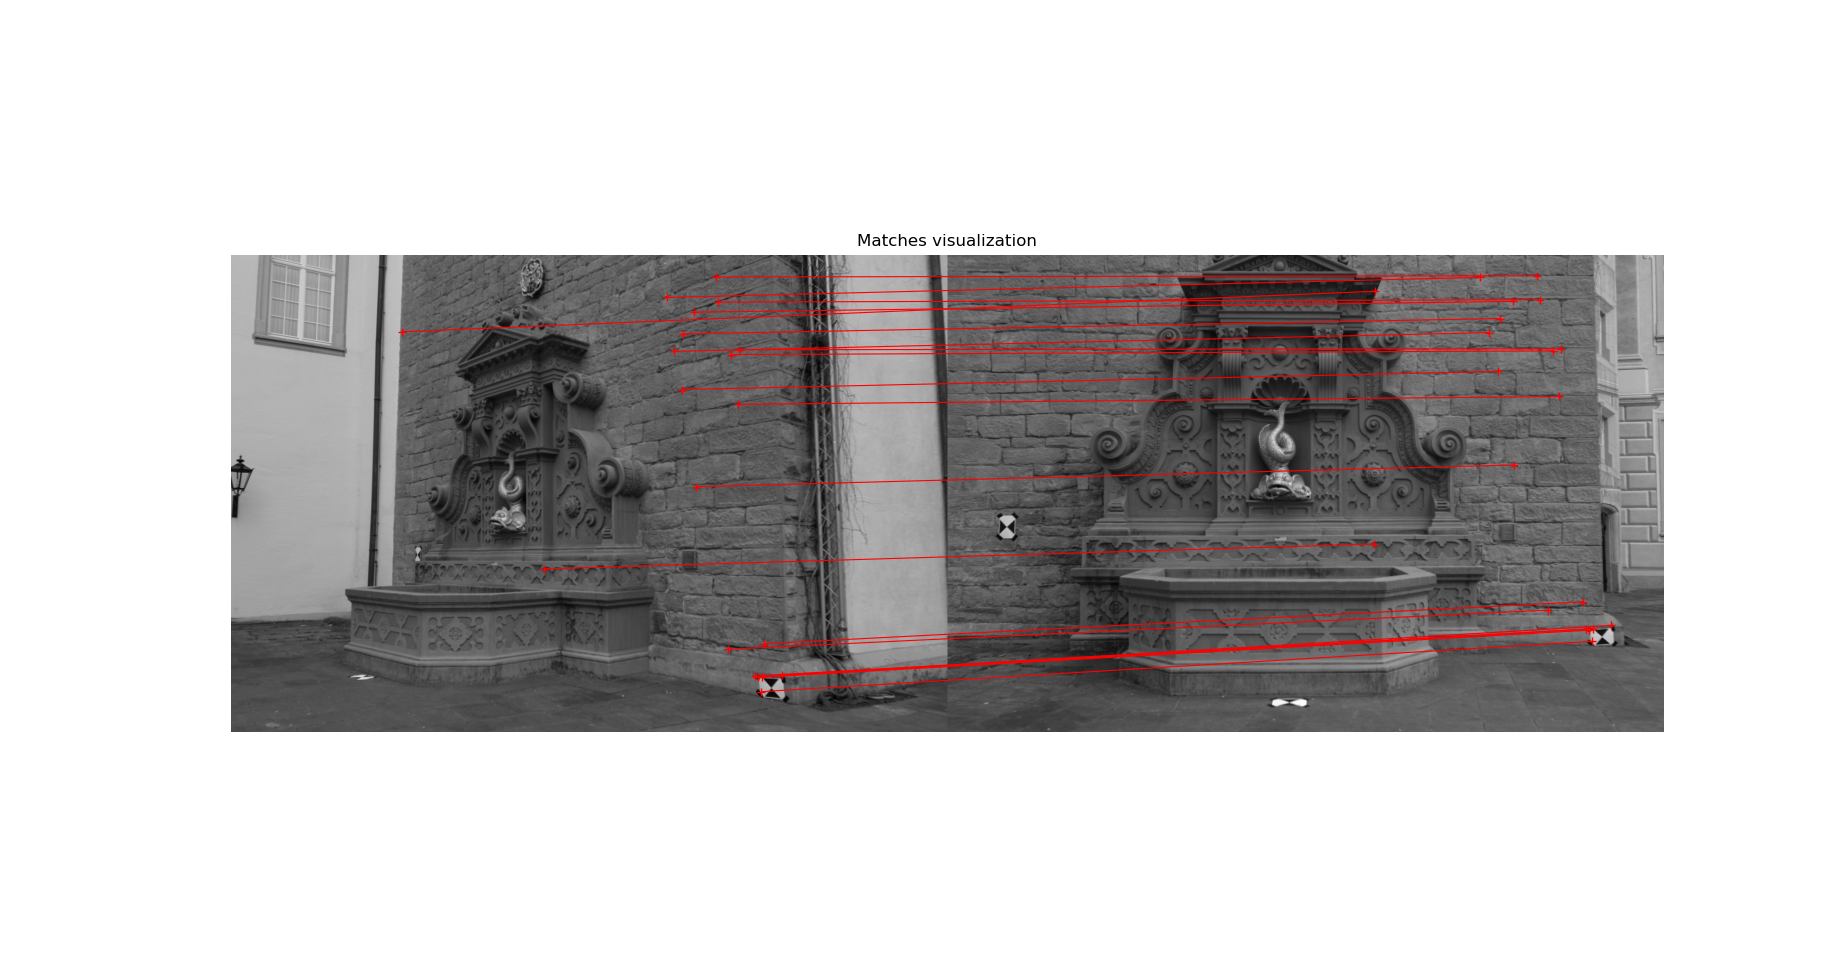
\includegraphics[width=1.0\linewidth]{putative_matches.png}
    \caption{Putative matches after passing Lowe's ratio test.}
    \label{fig:putative_matches}
\end{figure}


\end{quote}

\section*{Fundamental Matrix Estimation} 

\paragraph{Question 2 (Eight-point Estimation) [3 pts]:} Here you will be modifying "fundamental.py". For this question, your task is to implement the unnormalized eight-point algorithm (covered in class lecture) and normalized eight-point algorithm (\href{https://en.wikipedia.org/wiki/Eight-point_algorithm#Normalized_algorithm}{link}) to find out the fundamental matrix between two cameras. We provide code to compute the quality of your matrices based on the average geometric distance, i.e. the distance between each projected keypoint from one image to its corresponding epipolar line in the other image. Please report this distance in your pdf.

\paragraph{Answer:} 
\begin{quote}
Below is the code of eight-point algorithm estimating fundamental marix with either unnormalized by default or normalized version:

\begin{lstlisting}[language=Python, basicstyle=\scriptsize]
    def estimate_fundamental_matrix(matches, normalize=False):
    """
    Arguments:
        matches: Coords of matched keypoint pairs in image 1 and 2, dims (#matches, 4).
        normalize: Boolean flag for using normalized or unnormalized alg.
    Returns:
        F: Fundamental matrix, dims (3, 3).
    """
    F = np.eye(3)
    # --------------------------- Begin your code here
    assert len(matches) >= 8
    matches = matches.copy()

    A = np.empty((len(matches), 9))

    if normalize:
        all_p1_mean = matches[:,:2].mean(axis=0)
        all_p1_stdv = matches[:,:2].std(axis=0)
        all_p2_mean = matches[:,2:].mean(axis=0)
        all_p2_stdv = matches[:,2:].std(axis=0)

        # normalize points
        matches[:, :2] = (matches[:, :2] - all_p1_mean) / all_p1_stdv
        matches[:, 2:] = (matches[:, 2:] - all_p2_mean) / all_p2_stdv

        # construct transformation matrices
        T1 = np.eye(3)
        T1[:2, -1] -= all_p1_mean
        T1[:2, :] /= all_p1_stdv[:, np.newaxis]
        T2 = np.eye(3)
        T2[:2, -1] -= all_p2_mean
        T2[:2, :] /= all_p2_stdv[:, np.newaxis]
        
    # formulate a homogeneous linear equation
    for i, match in enumerate(matches):
        x1, y1, x2, y2 = match
        A[i] = [x2 * x1, x2 * y1, x2, y2 * x1, y2 * y1, y2, x1, y1, 1]
    
    # get solution to the constructed homogeneous linear equation (in the form of Af = 0)
    U, S, Vh = np.linalg.svd(A)
    # reshape the min singular value into a 3 by 3 matrix
    # (get f minimizing |Af|^2 subject to |f|^2 = 1)
    F = np.reshape(Vh[-1, :], (3, 3))   

    # enforce rank-2 constraint to the reconstructed fundamental matrix F
    U, S, Vh = np.linalg.svd(F)
    S[-1] = 0
    F = U @ np.diag(S) @ Vh
    
    # return to the original units with transformation matrices T1 and T2
    if normalize:
        F = T2.T @ F @ T1

    # --------------------------- End your code here
    return F
\end{lstlisting}

Note that rank-2 constraint is applied to enforce the estimated fundamental matrix to be rank-deficient. Also, be aware that the normalization mode involves recovering the estimate from the normalized to the original coordinate with the matrices \texttt{T1} and \texttt{T2} having the information on the mean and variance of the keypoints in the original images.

The performance of the implemented eight-point algorithm in both with and without normalization is evaluated as follow:

{\tt
F\_with\_normalization average geo distance: 0.01646852917832046 \\
F\_without\_normalization average geo distance: 0.023203213949373653
}

It is shown that the mode with normalization yields smaller average geometric distance, which is better. This is due to the virtue of normalization for a better conditioning in matrix operations.

\end{quote}

\paragraph{Question 3 (RANSAC) [3 pts]:} Here you will be modifying "fundamental.py". Your task is to implement RANSAC to find the fundamental matrix between two cameras. Please report the average geometric distance based on your estimated fundamental matrix, given 1, 100, and 10000 iterations of RANSAC. Please also visualize the inliers with your best estimated fundamental matrix in your solution for both images (we provide a visualization function). In your PDF, please also explain why we do not perform SVD or do a least-square over all the matched key points. 

\paragraph{Answer:} 
\begin{quote}

Below is the implementation of RANSAC estimating a fundamental matrix between images from the candidate matches of their keypoints:

\begin{lstlisting}[language=Python, basicstyle=\scriptsize]
def ransac(all_matches, num_iteration, estimate_fundamental_matrix, inlier_threshold):
    """
    Arguments:
        all_matches: coords of matched keypoint pairs in image 1 and 2, dims (# matches, 4).
        num_iteration: total number of RANSAC iteration
        estimate_fundamental_matrix: your normalized eight-point algorithm function
        inlier_threshold: threshold to decide if one point is inlier
    Returns:
        best_F: best Fundamental matrix, dims (3, 3).
        inlier_matches_with_best_F: (#inliers, 4)
        avg_geo_dis_with_best_F: float
    """

    best_F = np.eye(3)
    inlier_matches_with_best_F = None
    avg_geo_dis_with_best_F = 0.0

    ite = 0
    # --------------------------- Begin your code here

    while ite < num_iteration:
        ## step 1. obtain a fundamental matrix candidate
        # sample candidate matches randomly (at least eight-points are needed)
        num_samples = 8
        candidate_matches = all_good_matches[np.random.choice(len(all_good_matches), num_samples)]
        
        # estimate fundamental matrix of the candidate matches
        F = estimate_fundamental_matrix(candidate_matches, normalize=True)
        
        ## step 2. check the inliers by applying the estimated fundamental matrix to the whole matches
        # def apply_fundamental_matrix(F, matches):
        # transform the set of image points into homogeneous coordinates
        ones = np.ones((len(all_good_matches), 1))
        all_p1 = np.concatenate((all_good_matches[:, 0:2], ones), axis=1)
        all_p2 = np.concatenate((all_good_matches[:, 2:4], ones), axis=1)
        # get coefficients of epipolar lines
        # coefficients of epipolar lines appearing in img1 (corresponding to epipoles all_p1)
        F_p2 = np.dot(F.T, all_p2.T).T
        # coefficients of epipolar lines appearing in img2 (corresponding to epipoles all_p2)
        F_p1 = np.dot(F, all_p1.T).T
        # get geometric distances between reconstructed epipolar lines and corresponding epipoles
        p1_line2 = np.sum(all_p1 * F_p2, axis=1)[:, np.newaxis]
        p2_line1 = np.sum(all_p2 * F_p1, axis=1)[:, np.newaxis]
        # set of distances between the estimated epipolar lines (projected from p2) and epipoles (p1)
        dist_all_p1 = np.absolute(p1_line2) / np.linalg.norm(F_p2, axis=1)[:, np.newaxis]
        # set of distances between the estimated epipolar lines (projected from p1) and epipoles (p2)
        dist_all_p2 = np.absolute(p2_line1) / np.linalg.norm(F_p1, axis=1)[:, np.newaxis]
        dist_all = (dist_all_p1 + dist_all_p2) / 2

        # get indices of inliers
        inlier_idx = np.where(dist_all < inlier_threshold)[0]

        # step 3. update the best solution upon the number of inliers 
        if (inlier_matches_with_best_F is None) or (len(inlier_idx) > len(inlier_matches_with_best_F)):
            best_F = F
            inlier_matches_with_best_F = all_good_matches[inlier_idx]
            avg_geo_dis_with_best_F = dist_all.sum() / len(all_matches)

        ite += 1
    # --------------------------- End your code here
    return best_F, inlier_matches_with_best_F, avg_geo_dis_with_best_F
\end{lstlisting}

Note that the minimal number of keypoint pairs (i.e., eight) is used for estimatting a candidate fundamental matrix. I used the distance between a keypoint and its corresponding epipolar line reconstructed upon the estimated fundamental matrix candidate from one image to another (\texttt{dist\_all}) as a metric to count inlier (hence, its unit is in pixel); if the distance is smaller than the given threshold (\texttt{dist\_all < inlier\_threshold}), it counts as an inlier. This process is done for every iteration, while the candidate showing the most inliers is returned at the end. I used the threshold (\texttt{inlier\_threshold}) to be 1 by default; hence, the desired geometric distance between reconstructed epipolar lines and corresponding keypoints for both images is less than a pixel.

The reported average geometric distance between the keypoints and corresponding epipolar lines upon the estimated fundamental matrix with respect to the various number of RANSAC iterations is evaluated as follow:

{\tt
num\_iterations: 1e0; avg\_geo\_dis\_with\_best\_F: 0.12549801248070563; \\
num\_iterations: 1e2; avg\_geo\_dis\_with\_best\_F: 0.012038648914555196; \\
num\_iterations: 1e4; avg\_geo\_dis\_with\_best\_F: 0.02767357282414638;
}

Note that the average geometric distance (the smaller the better) does not improve a lot above at some \texttt{num\_iterations}, as RANSAC is a stochastic process depending on quality of the chosen matches for every iteration. For an edge case as an example, if the selected matches represents the underlying model best given the whole set of matches (hence, yielding the most inliers), the algorithm does not need to go over more iterations. 

Fig.~\ref{fig:ransac} is the visualized inlier keypoints with respect to the number of RANSAC iterations---1, 100, and 10000, respectively:

\begin{figure}[h]
    \centering
    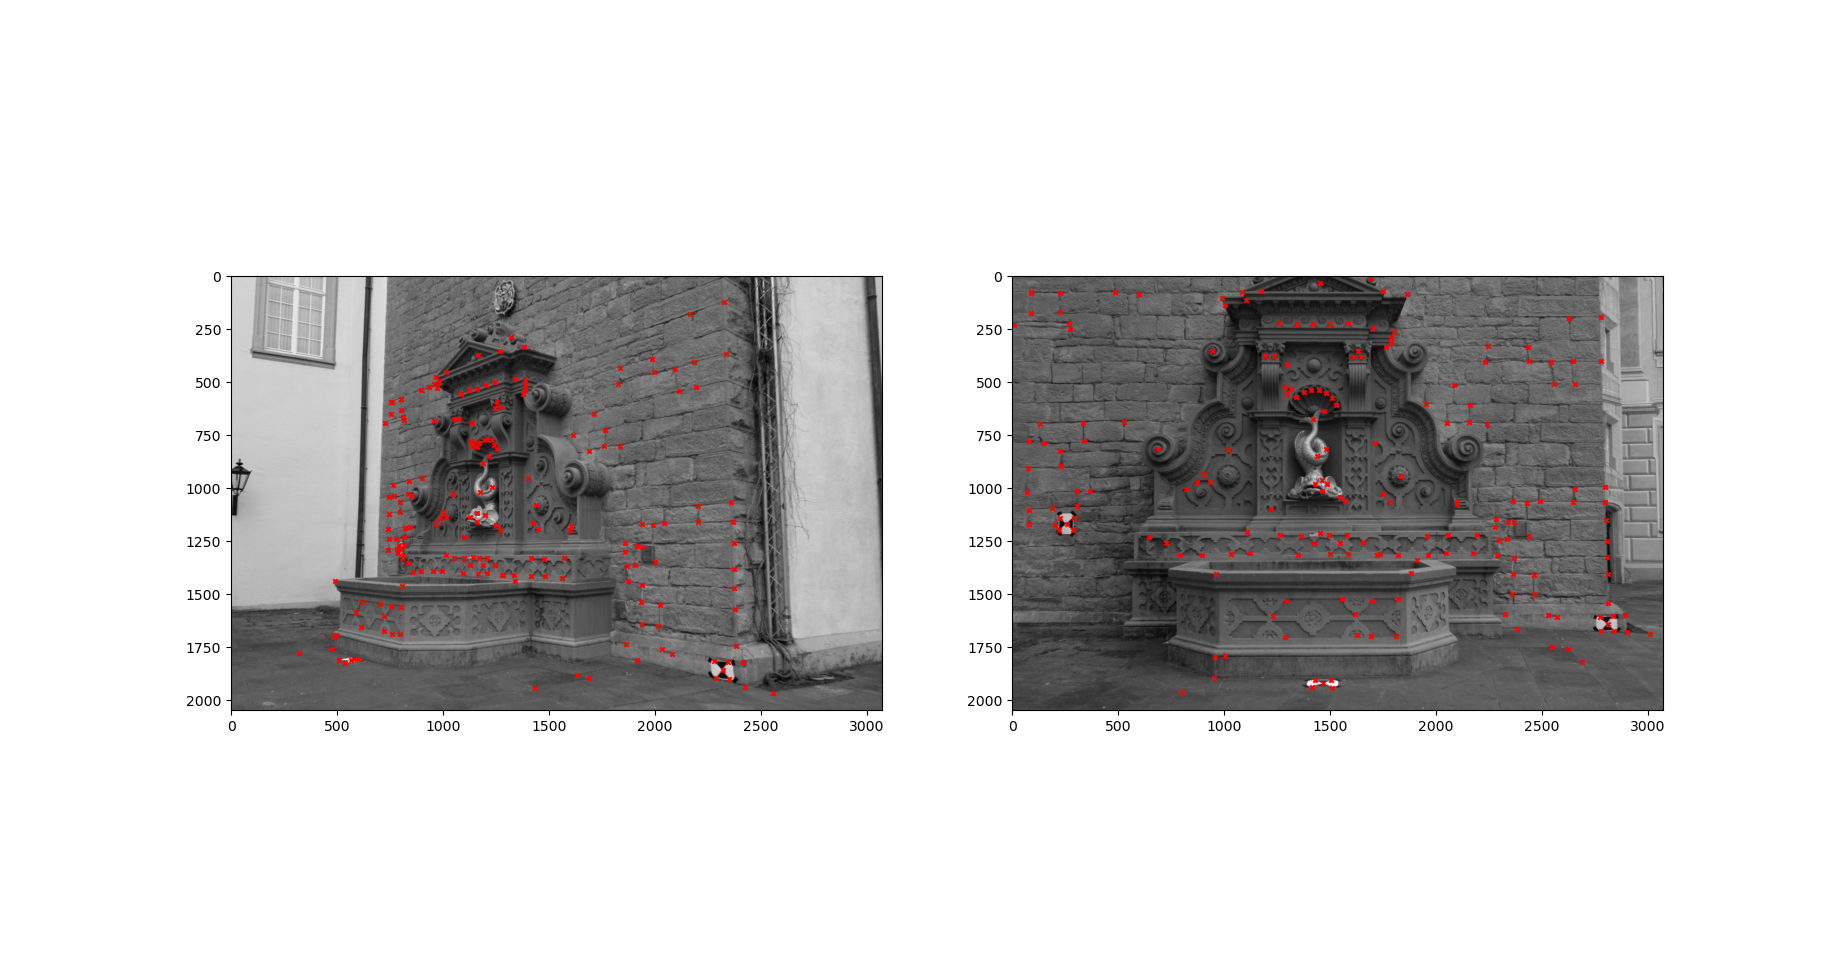
\includegraphics[height=7.5cm]{ransac_num_iter_1e0.png} % width=1.0\linewidth
    \caption{Inlier keypoints with the estimated fundamental matrix from RANSAC (iteration: 1e0)}
    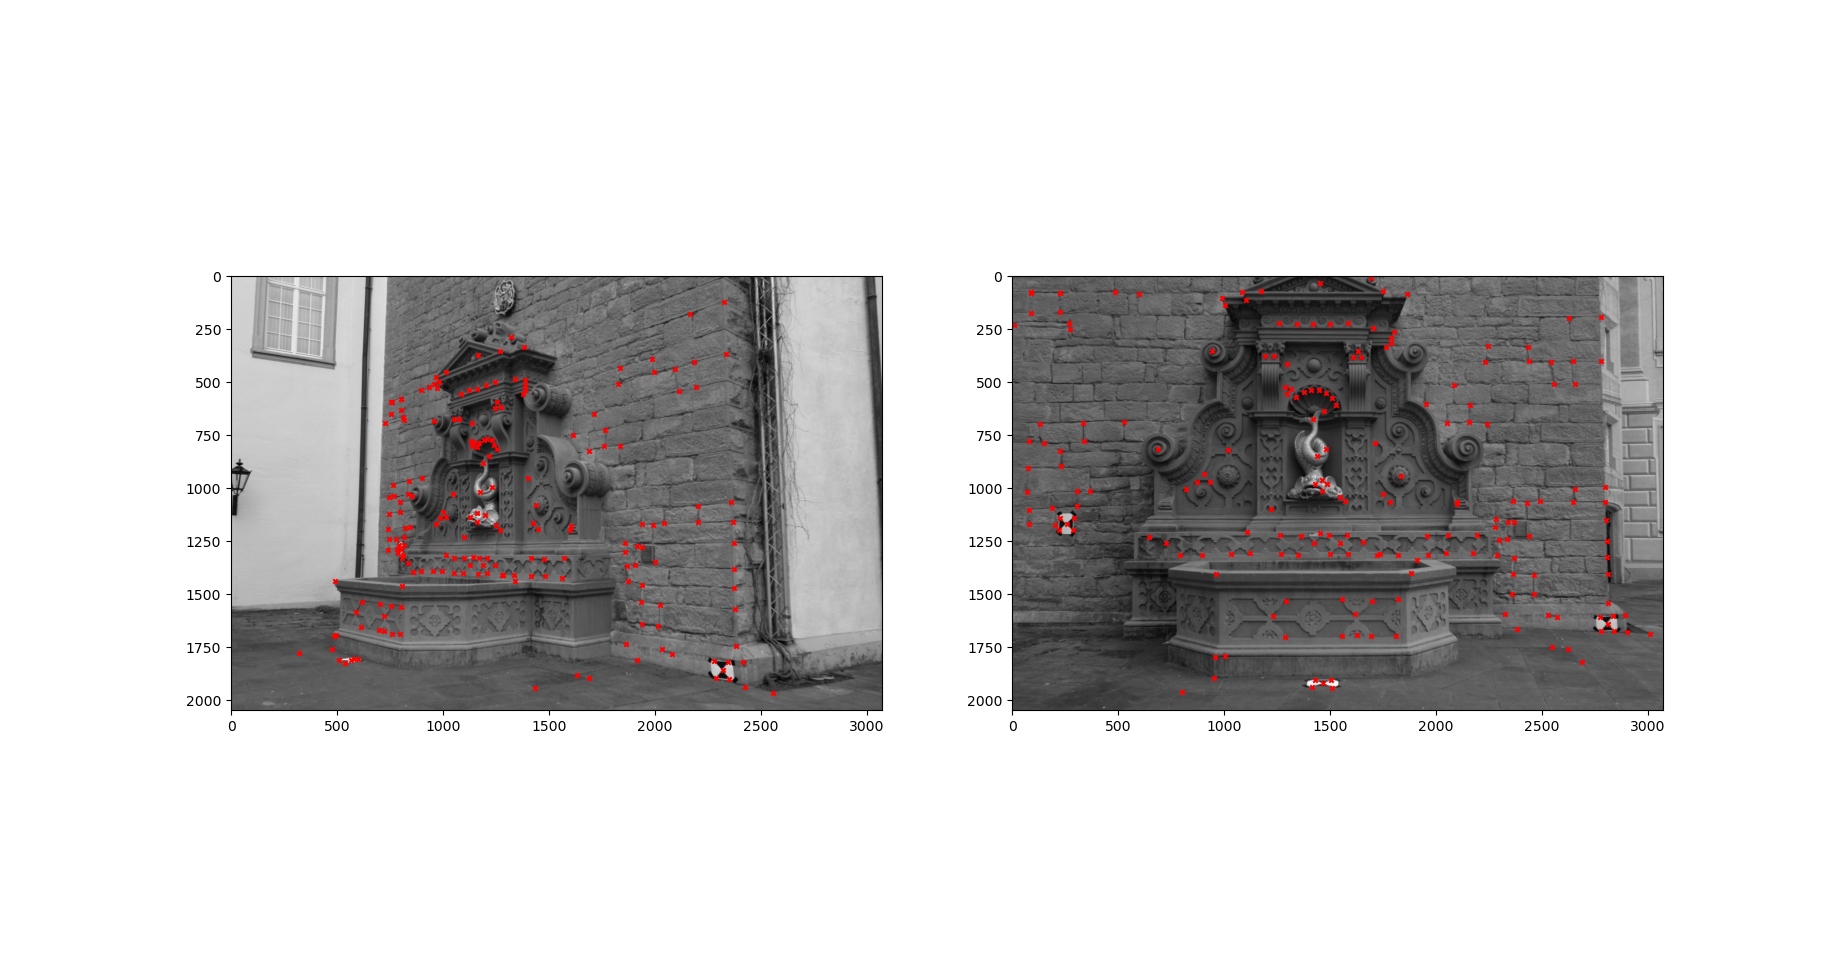
\includegraphics[height=7.5cm]{ransac_num_iter_1e2.png}
    \caption{Inlier keypoints with the estimated fundamental matrix from RANSAC (iteration: 1e2)}
    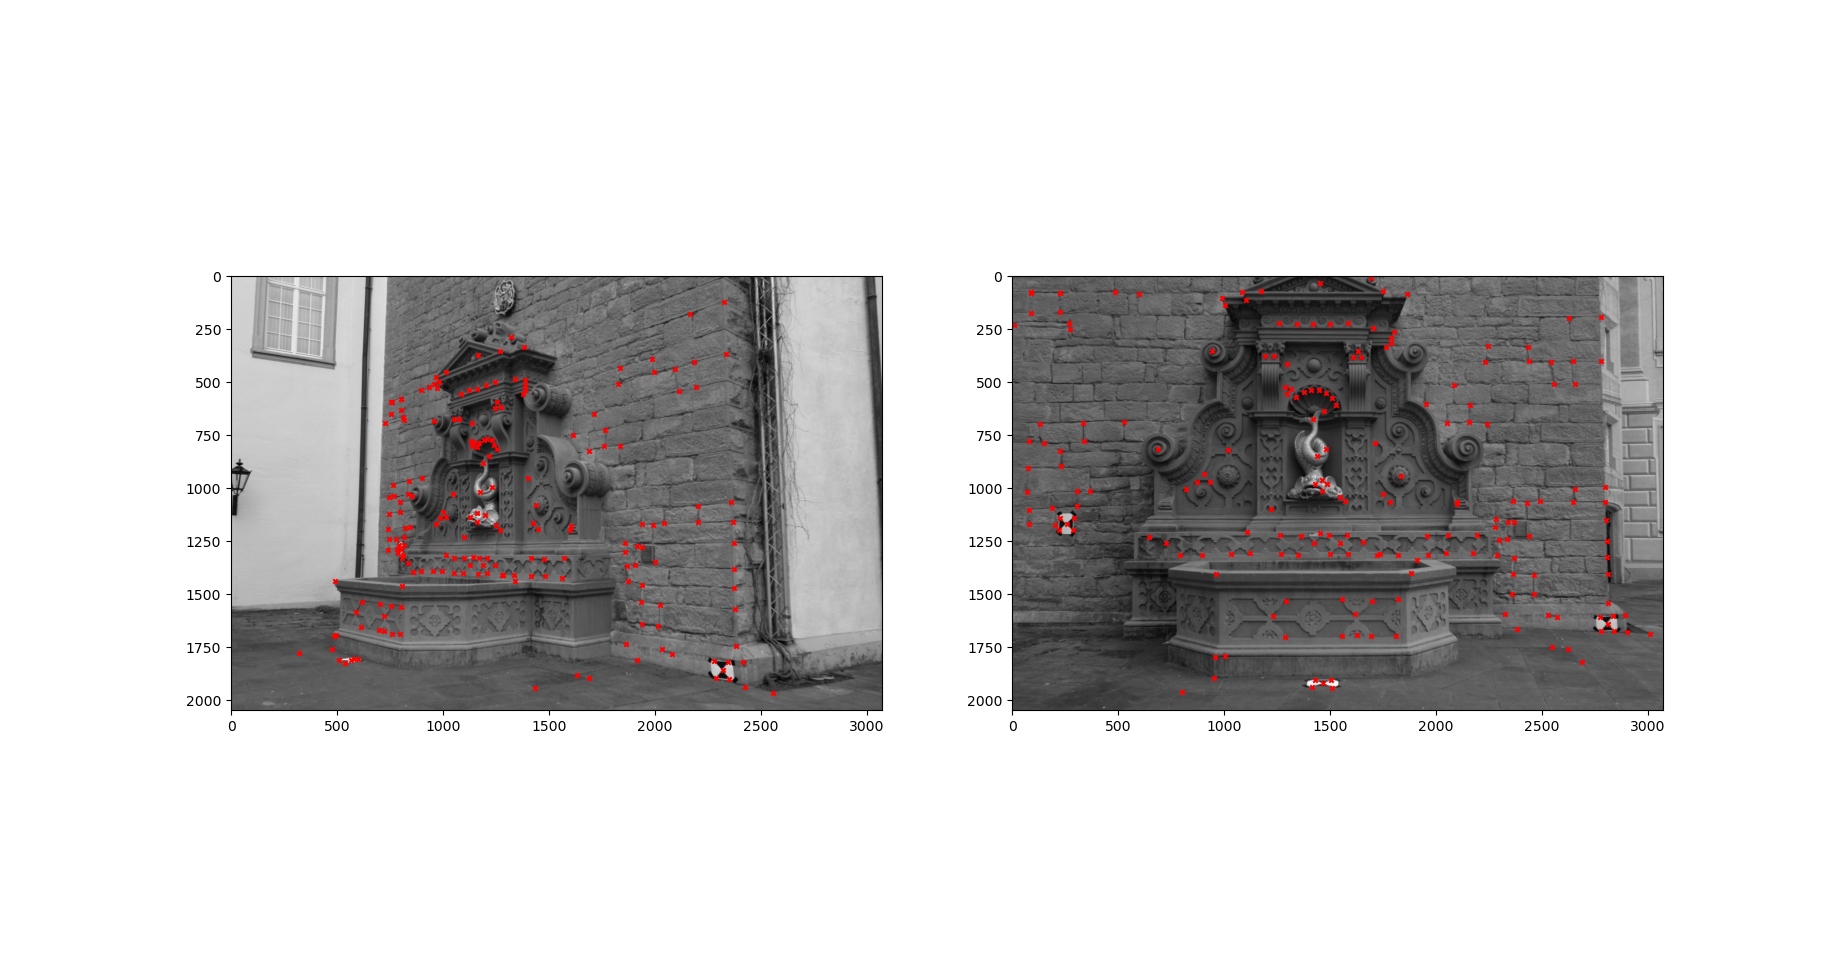
\includegraphics[height=7.5cm]{ransac_num_iter_1e4.png}
    \caption{Inlier keypoints with the estimated fundamental matrix from RANSAC (iteration: 1e4)}
    \label{fig:ransac}
\end{figure}


The reason why not doing the fundamental matrix estimation over the whole matches is twofold. First, getting the solution of a homogeneous system of equation become extremely expensive with a large number of data, as the cost of SVD increases cubically with respect to the size of matrix. Second, the estimate may not respresent the model well in the case when the portion of inliers is not negligible, which is because either an inlier or an outlier is equally considered in a normal least-square problem. For this reasons, the suggested RANSAC algorithm---estimating the candidate over chosen data, counting inliers, and saving the best one---is used, instead of running the eight-point algorithm over the whole matching pairs.

\end{quote}

\paragraph{Question 4 (Epipolar Line Visualization) [1 pt]:} Here you will be modifying "fundamental.py". Please visualize the epipolar line for both images for your estimated F in Q2 and Q3. Here we do not provide you visualization code. To draw on images, cv2.line, cv2.circle are useful for plotting lines and circles. Check our Lecture 4, Epipolar Geometry, to learn more about equation of epipolar line. This \href{https://web.stanford.edu/class/cs231a/course_notes/03-epipolar-geometry.pdf}{link} also gives a thorough review of epipolar geometry.

\paragraph{Answer:} 
\begin{quote}

Below is the function visualizing the keypoints and corresponding epipolar line estimates from the one image to the other given the fundamental matrix on both images:

\begin{lstlisting}[language=Python, basicstyle=\scriptsize]
def visualize(estimated_F, img1, img2, kp1, kp2):
    # --------------------------- Begin your code here
    assert len(kp1) == len(kp2)
    
    all_p1 = np.concatenate((kp1, np.ones((len(kp1),1))), axis=1)
    all_p2 = np.concatenate((kp2, np.ones((len(kp2),1))), axis=1)
    
    # coefficients of epipolar lines appearing in img1 (corresponding to epipoles all_p1)
    F_p2 = np.dot(estimated_F.T, all_p2.T).T
    # coefficients of epipolar lines appearing in img2 (corresponding to epipoles all_p2)
    F_p1 = np.dot(estimated_F, all_p1.T).T    

    # get geometric distances between reconstructed epipolar lines and corresponding epipoles
    p1_line2 = np.sum(all_p1 * F_p2, axis=1)[:,np.newaxis]
    p2_line1 = np.sum(all_p2 * F_p1, axis=1)[:,np.newaxis]

    # set of distances between the estimated epipolar lines (projected from p2) and epipoles (p1)
    dist_all_p1 = np.absolute(p1_line2) / np.linalg.norm(F_p2, axis=1)[:,np.newaxis]
    # set of distances between the estimated epipolar lines (projected from p1) and epipoles (p2)
    dist_all_p2 = np.absolute(p2_line1) / np.linalg.norm(F_p1, axis=1)[:,np.newaxis]

    # get points on every reconstructed line closest to the corresponding epipole
    all_p1_closest = kp1 - F_p2[:,:2] / np.linalg.norm(F_p2[:,:2], axis=1)[:,np.newaxis] \
                           * np.einsum('ij,ij->i', all_p1, F_p2)[:,np.newaxis]
    all_p2_closest = kp2 - F_p1[:,:2] / np.linalg.norm(F_p1[:,:2], axis=1)[:,np.newaxis] \
                           * np.einsum('ij,ij->i', all_p2, F_p1)[:,np.newaxis]

    # find endpoints of segment on every epipolar line
    # offset from the closest point is 100 pixels
    l = 100
    all_p1_src = all_p1_closest + np.hstack((F_p2[:,1][:,np.newaxis], -F_p2[:,0][:,np.newaxis])) \
                                  / np.linalg.norm(F_p2[:,:2], axis=1)[:, np.newaxis] * l
    all_p1_dst = all_p1_closest - np.hstack((F_p2[:,1][:,np.newaxis], -F_p2[:,0][:,np.newaxis])) \
                                  / np.linalg.norm(F_p2[:,:2], axis=1)[:, np.newaxis] * l
    all_p2_src = all_p2_closest + np.hstack((F_p1[:,1][:,np.newaxis], -F_p1[:,0][:,np.newaxis])) \
                                  / np.linalg.norm(F_p1[:,:2], axis=1)[:, np.newaxis] * l
    all_p2_dst = all_p2_closest - np.hstack((F_p1[:,1][:,np.newaxis], -F_p1[:,0][:,np.newaxis])) \
                                  / np.linalg.norm(F_p1[:,:2], axis=1)[:, np.newaxis] * l

    # Display points and segments of corresponding epipolar lines.
    # You will see points in red corsses, epipolar lines in green 
    # and a short cyan line that denotes the shortest distance between
    # the epipolar line and the corresponding point.
    
    plt.tight_layout()

    plt.subplot(1, 2, 1)
    plt.imshow(img1, cmap='gray')
    plt.plot(kp1[:,0], kp1[:,1],  '+r')
    plt.plot([kp1[:,0], all_p1_closest[:,0]],[kp1[:,1], all_p1_closest[:,1]], 'r')
    plt.plot([all_p1_src[:,0], all_p1_dst[:,0]],[all_p1_src[:,1], all_p1_dst[:,1]], 'g')
    plt.xlim(0, img1.shape[1])
    plt.ylim(img1.shape[0], 0)

    plt.subplot(1, 2, 2)
    plt.imshow(img2, cmap='gray')
    plt.plot(kp2[:,0], kp2[:,1],  '+r')
    plt.plot([kp2[:,0], all_p2_closest[:,0]],[kp2[:,1], all_p2_closest[:,1]], 'r')
    plt.plot([all_p2_src[:,0], all_p2_dst[:,0]],[all_p2_src[:,1], all_p2_dst[:,1]], 'g')
    plt.xlim(0, img2.shape[1])
    plt.ylim(img2.shape[0], 0)
    
    plt.show()
    # --------------------------- End your code here
\end{lstlisting}

First, the (unnormalized) coefficients of epipolar lines that will appear in both img1 and img2 for every keypoint are calculated (\texttt{F\_p2}, \texttt{F\_p1}). Unfortunately, those epipolar lines do not prefectly pass through their desired eipoles (\texttt{kp1}, \texttt{kp2}) due to the imperfectness of the estimated fundamental matrices---hence, the points on the epipolar lines closest to their corresponding keypoints are calculated (\texttt{all\_p1\_closest}, \texttt{all\_p2\_closest}). The line segments around these points are then estimated, whose starting and ending points are \texttt{all\_p1\_src}, \texttt{all\_p2\_src} and \texttt{all\_p1\_dst}, \texttt{all\_p2\_dst}, respectively. Then the keypoints, epipolar line segments, and their closest distances are colored in red, green, and cyan in both images. The outcomes are in Fig.~\ref{fig:epipolar_lines_8pts} and Fig.~\ref{fig:epipolar_lines_ransac}, where each case uses the fundamental matrix estimated from the eight-point algorithm (in Q2) and RANSAC (in Q3).

\begin{lstlisting}[language=Python, basicstyle=\scriptsize]
F_Q2 = F_with_normalization # estimated F in Q2
F_Q3 = best_F               # estimated F in Q3
\end{lstlisting}


\begin{figure}[h]
    \centering
    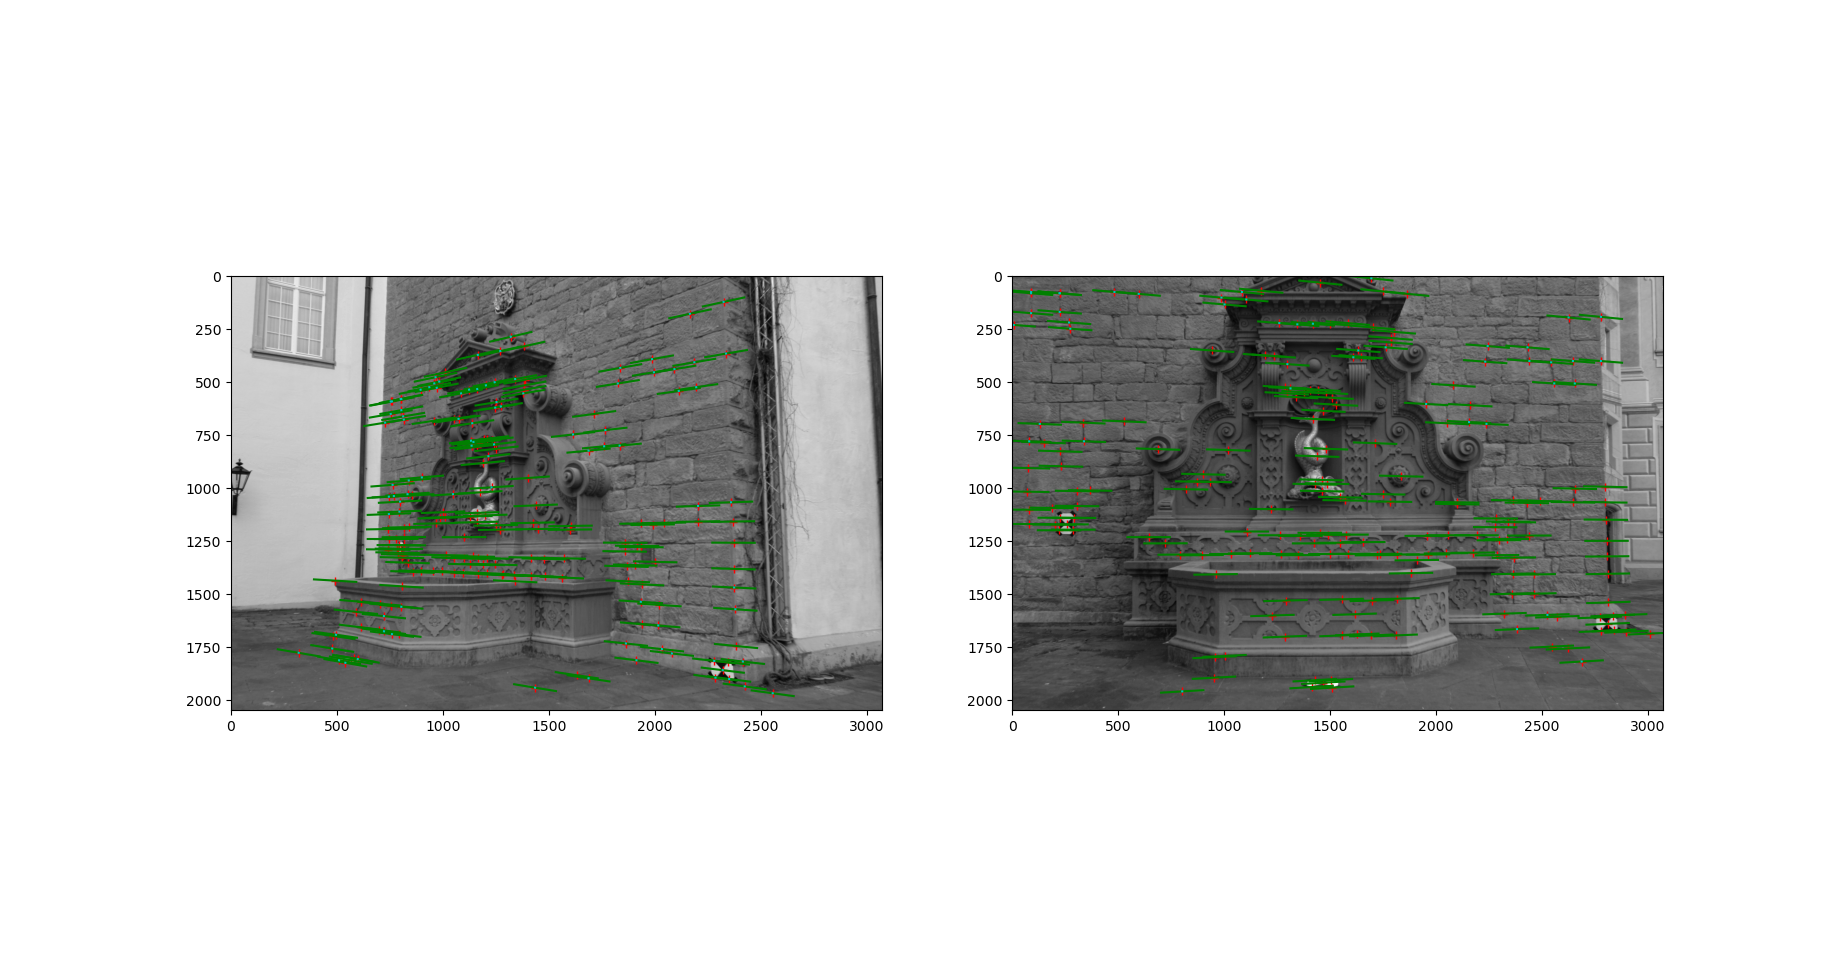
\includegraphics[width=1.0\linewidth]{epipolar_lines_8pts.png}
    \caption{Keypoints and epipolar lines from a fundamental matrix estimated by eight-point algorithm}
    \label{fig:epipolar_lines_8pts}
\end{figure}

\begin{figure}[h]
    \centering
    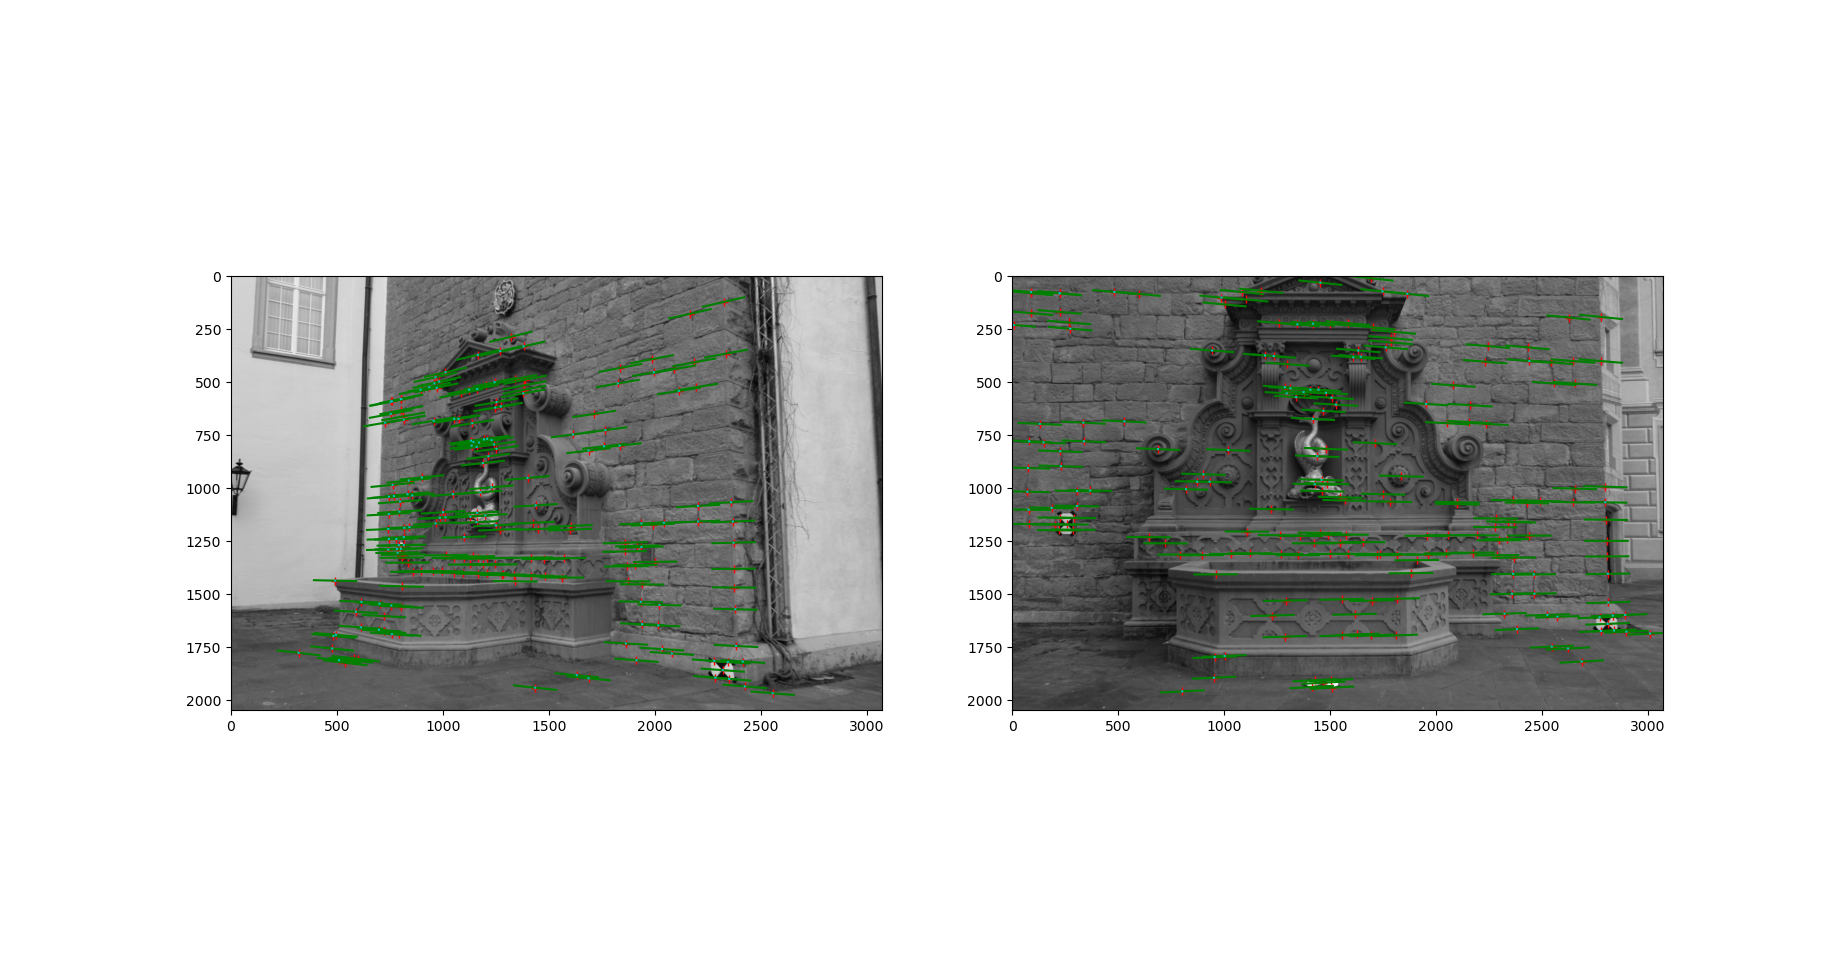
\includegraphics[width=1.0\linewidth]{epipolar_lines_ransac.png}
    \caption{Keypoints and epipolar lines from a fundamental matrix estimated by RANSAC}
    \label{fig:epipolar_lines_ransac}
\end{figure}


\end{quote}

\section*{Unprojection} 
After solving relative poses between our two cameras, now we will move from 2d to 3d space.

\paragraph{Question 5 (Triangulation) [3 pts]:}
Here you will be modifying "triangulation.py". You are given keypoint matching between two images, together with the camera intrinsic and extrinsic matrix. Your task is to perform triangulation to restore the 3D coordinates of the key points. In your PDF, please visualize the 3d points and camera poses in 3D from different viewing perspectives. 

\paragraph{Answer:} 
\begin{quote}

Below is the function performing triangulation for every matching pair and returning its estimated location in 3-D coordinate given camera intrinsic and extrinsic matrices:

\begin{lstlisting}[language=Python, basicstyle=\scriptsize]
def triangulate(K1, K2, R1, R2, t1, t2, all_good_matches):
    """
    Arguments:
        K1: intrinsic matrix for image 1, dim: (3, 3)
        K2: intrinsic matrix for image 2, dim: (3, 3)
        R1: rotation matrix for image 1, dim: (3, 3)
        R2: rotation matrix for image 1, dim: (3, 3)
        t1: translation for image 1, dim: (3,)
        t2: translation for image 1, dim: (3,)
        all_good_matches:  dim: (#matches, 4)
    Returns:
        points_3d, dim: (#matches, 3)
    """
    points_3d = None
    # --------------------------- Begin your code here
    # credit: http://www.cs.cmu.edu/~16385/s17/Slides/11.4_Triangulation.pdf

    # cosntruct camera projection matrix
    T1 = np.eye(4); T1[:3, :3] = R1; T1[:3, -1] = t1.flatten()
    T2 = np.eye(4); T2[:3, :3] = R2; T2[:3, -1] = t2.flatten()
    eye_3by4 = np.zeros((3,4)); eye_3by4[:, :3] = np.eye(3)
    M1 = K1 @ eye_3by4 @ T1
    M2 = K2 @ eye_3by4 @ T2

    # container for the estimated 3d points reconstructed by triangulation
    points_3d = np.empty((len(all_good_matches), 3))
    
    for i, match in enumerate(all_good_matches):
        # conduct triangulation of the given 2d matches
        x1, y1, x2, y2 = match
        A = np.vstack((y1 * M1[2,:] -      M1[1,:],
                            M1[0,:] - x1 * M1[2,:],
                       y2 * M2[2,:] -      M2[1,:],
                            M2[0,:] - x2 * M2[2,:]))
        U, S, Vh = np.linalg.svd(A)
        pt_3d = np.reshape(Vh[-1, :], (4,))
        pt_3d /= pt_3d[-1]

        # save to the array
        points_3d[i] = pt_3d[:-1]

    # --------------------------- End your code here
    return points_3d
\end{lstlisting}

The basic logic is simlar to what we did for the previous tasks, with a slightly different formulation of the system of equations.

Below is the code visualizing both estimated keypoints in 3-D coordinate along with the cameras' locations. Be aware that general Matplotlib functions are used instead of Open3D:

\begin{lstlisting}[language=Python, basicstyle=\scriptsize]
# --------------------------- Begin your code here
# obtain camera center in 3D world frame
cam1 = - R1.T @ t1
cam2 = - R2.T @ t2

cam1 = cam1.flatten()
cam2 = cam2.flatten()

camera_centers = np.vstack((cam1, cam2))

fig = plt.figure()
ax = fig.add_subplot(111, projection='3d')
ax.scatter(points_3d[:, 0], points_3d[:, 1], points_3d[:, 2], c='b', label='Points')
ax.scatter(camera_centers[:, 0], camera_centers[:, 1], camera_centers[:, 2], \
           c='g', s=50, marker='^', label='Camera Centers')
ax.legend(loc='best')

plt.show()

\end{lstlisting}

Note that the the center of camera in the given 3D world frame is estimated. The estimated 3-D keypoints (\texttt{points\_3d}) along with cameras (\texttt{cam1}, \texttt{cam2}) are shown in Fig.~\ref{fig:triangulation}.

\begin{figure}[h]
    \centering
    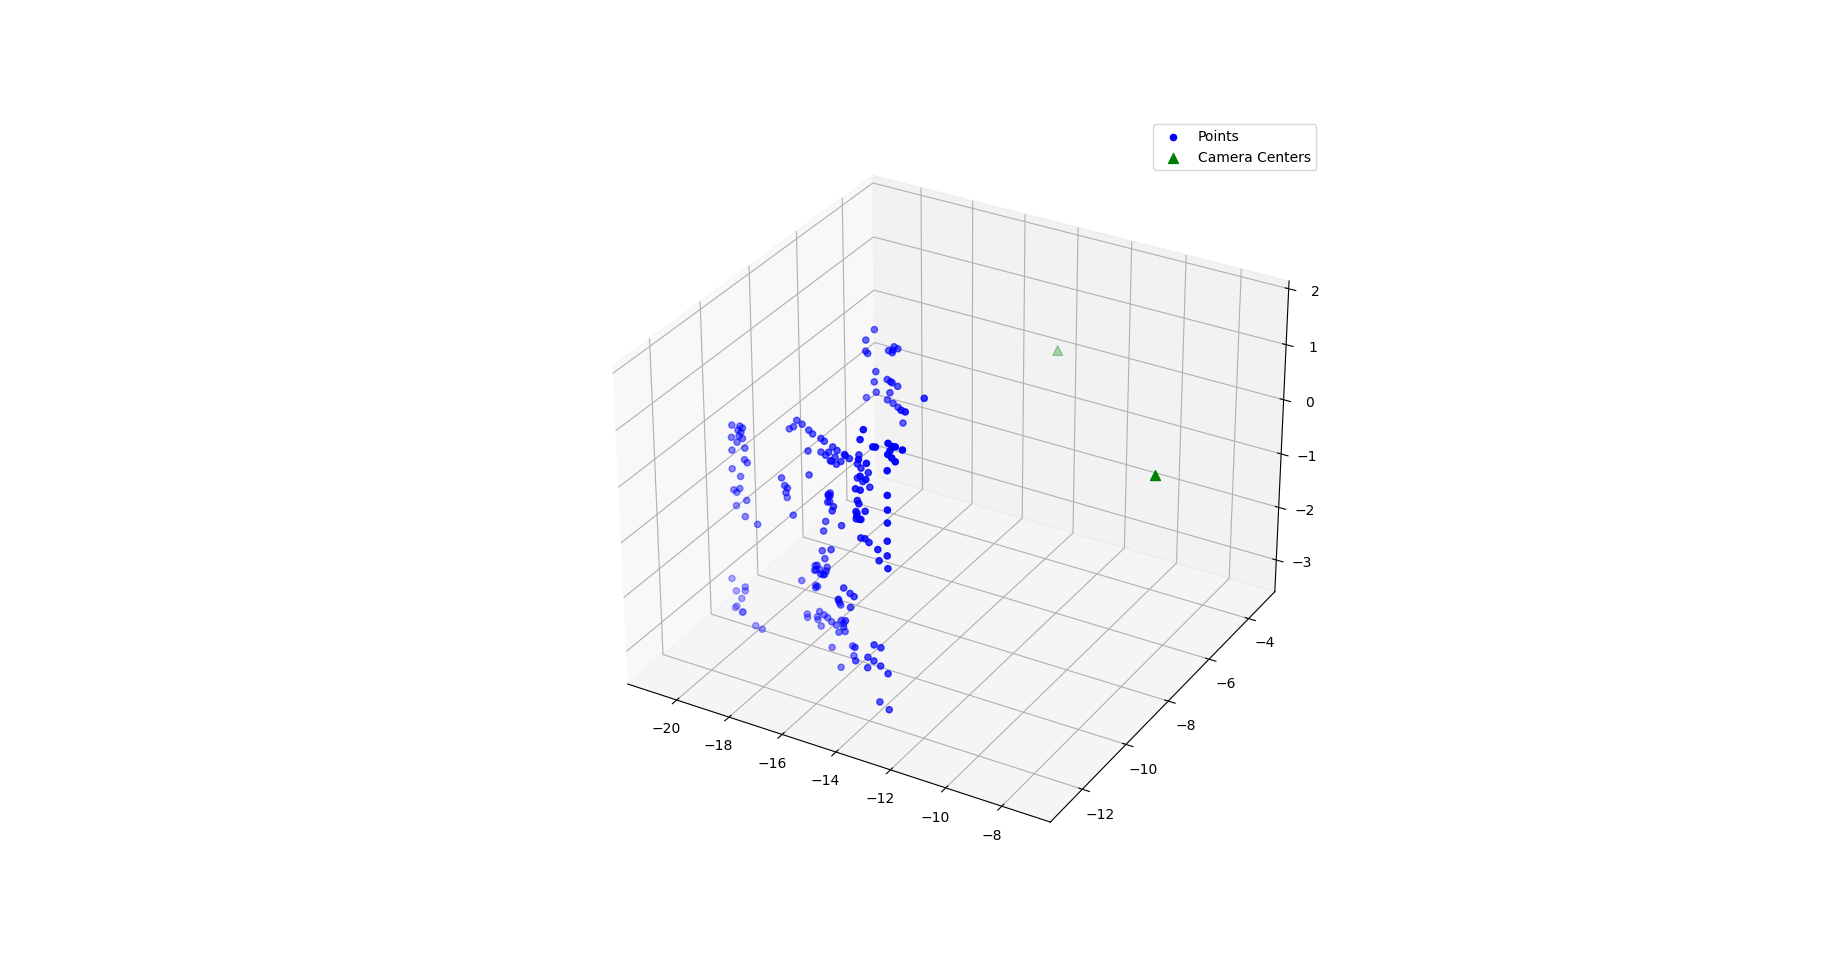
\includegraphics[width=1.0\linewidth]{triangulation.png}
    \caption{Keypoints estimated by triangulation along with cameras in a 3-D frame}
    \label{fig:triangulation}
\end{figure}

\end{quote}

\section*{Stereo Estimation}

Now given two camera poses, we could get the relative camera pose and a sparse set of 3D point based on sparse keypoint matching. Could we go further and recover the dense geometry? The answer is yes. In question 6, you will reason a dense point cloud from a pair of images taken at the different views. 


\paragraph{Question 6 (Stereo) [3 pts + 1 bonus pt]:}
Given two images ($\mathbf{I}_1, \mathbf{I}_2$) with ground-truth intrinsic matrices $\mathbf{K}_1, \mathbf{K}_2$, extrinsic matrices $\mathbf{R}_1, \mathbf{t}_1, \mathbf{R}_2, \mathbf{t}_1$. Our goal is to recover a dense correspondence between the two images using stereo matching. 

Computing the dense matching is computationally expensive. We down-sample both images by $s$ times to reduce the computational burden. Could you describe what will be the updated intrinsic matrices? Please report the intrinsics on your write-up and fill in the code to update $\mathbf{K}_1, \mathbf{K}_2$. 

\paragraph{Answer:} 
\begin{quote}

The camera intrinsic parameters---focal lengths ($f_u$, $f_v$) and offsets of the principal point ($p_u$, $p_v$) ---are downscaled as the original image shrinks down, which is done by as below:

\begin{lstlisting}[language=Python, basicstyle=\scriptsize]
K1[:2, :] //= scale
K2[:2, :] //= scale
\end{lstlisting}

It results in new intrinsic matrices as below:

\begin{lstlisting}[language=Python, basicstyle=\scriptsize]
K1 (unscaled): 
[[2759.48    0.   1520.69]
[   0.   2764.16 1006.81]
[   0.      0.      1.  ]]
K2 (unscaled): 
[[2759.48    0.   1520.69]
[   0.   2764.16 1006.81]
[   0.      0.      1.  ]]
K1 (scaled): 
[[344.   0. 190.]
[  0. 345. 125.]
[  0.   0.   1.]]
K2 (scaled): 
[[344.   0. 190.]
[  0. 345. 125.]
[  0.   0.   1.]]
\end{lstlisting}
    
\end{quote}

We do notice that the pair of images are not perfectly fronto-parallel. To make matching easier, we will rectify the pair of images such that its epipolar lines are always horizontal. To achieve this, we simply call \texttt{cv2.StereoRectify} function. The updated projection matrices are also returned. Please go through the code and understand what each step does. You do not need to write any code here. 

Finally, we will do stereo matching. Specifically, given a pixel at $(i, j)$ on the left image, we will compute a winner-take-all disparity value that minimizes the sum of square distance (SSD) between a pair of left and right image patches, centered at $(i, j)$ and $(i, j-d)$: 
\[
d[i, j] = \arg\min_d \sum_{m=-w}^{w} \sum_{n=-w}^{w} ( I_1[i+m, j+n] - I_2[i+m, j+n-d] )^2
\]
where $w*2+1$ is the block size and $w$ is an integer. Please do this in a sliding window manner to get the dense disparity map. Please visualize the disparity map you get and include it in your report.

\paragraph{Answer:} 
\begin{quote}

Below is the code of stereo matching given a rectified image pair.

\begin{lstlisting}[language=Python, basicstyle=\tiny]
def stereo_matching_ssd(left_im, right_im, max_disp=128, block_size=21):
    """
    Using sum of square difference to compute stereo matching.
    Arguments:
        left_im: left image (h x w x 3 numpy array)
        right_im: right image (h x w x 3 numpy array)
        mask_disp: maximum possible disparity
        block_size: size of the block for computing matching cost
    Returns:
        disp_im: disparity image (h x w numpy array), storing the disparity values
    """
    # --------------------------- Begin your code here
    assert left_im.shape == right_im.shape
  
    # convert to grayscale
    left_gray = cv2.cvtColor(left_im, cv2.COLOR_BGR2GRAY)
    right_gray = cv2.cvtColor(right_im, cv2.COLOR_BGR2GRAY)
    
    h, w = left_gray.shape
    
    # create padded arrays
    left_gray_padded = np.zeros((h+block_size-1,w+block_size-1), dtype=left_gray.dtype)
    right_gray_padded = np.zeros((h+block_size-1,w+block_size-1,max_disp), dtype=right_gray.dtype)
    
    left_gray_padded[block_size//2:h+block_size//2, block_size//2:w+block_size//2] = left_gray
    for d in range(max_disp):
      right_gray_padded[block_size//2:h+block_size//2, block_size//2+d:w+min(block_size-1, block_size//2+d), d] =\
         right_gray[:, :w+min(block_size-1, block_size//2+d)-block_size//2-d]
  
    # create strided arrays
    # left_gray_strided[j,i] indicates (block_size, block_size) np.array around left_gray[i,j]
    # right_gray_strided[j,i,d] indicates (block_size, block_size) np.array around right_gray[i,j]
    from numpy.lib.stride_tricks import as_strided
  
    left_gray_strided = np.empty(shape=left_gray.shape+(block_size,block_size), dtype=left_gray.dtype)
    right_gray_strided = np.empty(shape=right_gray.shape+(max_disp,)+(block_size,block_size), dtype=right_gray.dtype)
  
    left_gray_strided = as_strided(left_gray_padded, shape=left_gray.shape+(block_size,block_size), strides=left_gray_padded.strides*2)
    for d in range(max_disp):
      right_gray_strided[:,:,d,:,:] = as_strided(right_gray_padded[:,:,d], shape=right_gray.shape+(block_size,block_size), strides=right_gray_padded.strides[:-1]*2)
  
    # compute squared sum of distance
    # disp_map_candidate[j,i,d] indicates the ssd at (j,i) with a disparity offset d
    disp_map_candidate = np.empty(shape=left_gray.shape+(max_disp,), dtype=np.int64)
    for d in range(max_disp):
      for j in range(h):
        for i in range(w):
          disp_map_candidate[j,i,d] = ((left_gray_strided[j,i] - right_gray_strided[j,i,d])**2).sum()
    
  
    # extract disparity
    # disp_map[j,i] indicates the disparity of two images at (j,i)
    disp_map = np.argmin(disp_map_candidate, axis=2)
    
    # to avoid zero-division, covert zero elements to be -1
    disp_map[np.where(disp_map==0)] = -1
    disp_map = disp_map.astype(np.float64)
  
    # --------------------------- End your code here
    return disp_map
\end{lstlisting}

First, zero-padded grayscale images (\texttt{left\_gray\_padded}, \texttt{right\_gray\_padded}) with a margine of \texttt{block\_size} are created. Then numpy arrays \texttt{left\_gray\_strided} and \texttt{right\_gray\_strided}---with shapes \texttt{(H,W,B,B)} and \texttt{(H,W,D,B,B)} (\texttt{H}: image height, \texttt{W}: image width, \texttt{B}: block size, \texttt{D}: maximum disparity) respectively, are generated. These strided arrays are intended to facilitate block matching operation for every pixel and offset in a brute-force manner. \texttt{left\_gray\_strided[j,i]} indicates (\texttt{block\_size}, \texttt{block\_size}) np.array around \texttt{left\_gray[j,i]}, and \texttt{right\_gray\_strided[j,i,d]} indicates (\texttt{block\_size}, \texttt{block\_size}) np.array around \texttt{left\_gray[j,i]} with an offset by \texttt{d}. After then, squared sums of distance (SSD) for every pixel and offset are calculated in an numpy array \texttt{disp\_map\_candidate} with a shape \texttt{(H,W,B)}, where \texttt{disp\_map\_candidate[y,x,d]} indicates the SSD at \texttt{(j,i)} with a disparity offset \texttt{d}. Then the offset resulting in the minimum SSD for every pixel is obtained and saved in an array \texttt{disp\_map}. 

Fig.~\ref{fig:disparity_ssd} shows the estimated disparity map from our implementation.

\begin{figure}[h]
    \centering
    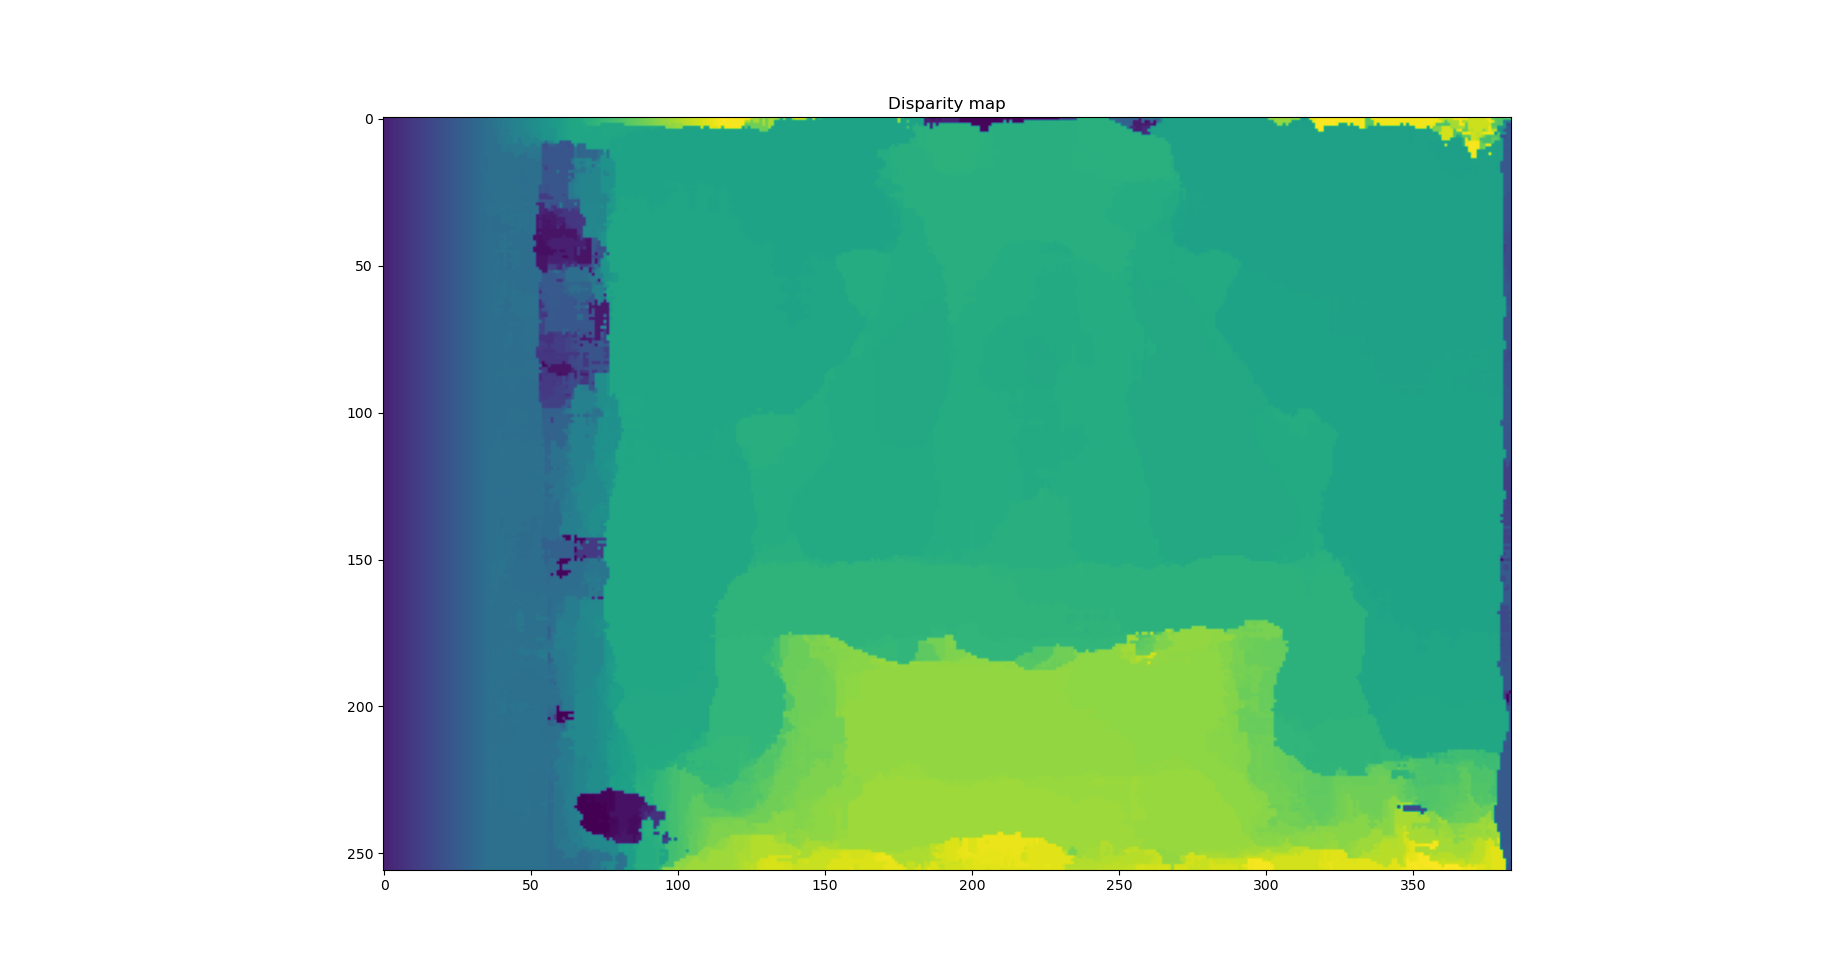
\includegraphics[width=1.0\linewidth]{disparity_ssd.png}
    \caption{Disparity estimates from our implementation.}
    \label{fig:disparity_ssd}
\end{figure}

\end{quote}

Do you think the disparity you get is satisfactory? You could compare your results against stereo matching results implemented by an off-the-shelf method \texttt{cv2.stereoBM} (we already provide the code). Visualize both methods side-by-side and provide insights into further improving your results. Given disparity map estimation, could you get the dense point cloud? Try to get the point cloud and visualize your point cloud.  (Bonus 1 pt)

\paragraph{Answer:} 
\begin{quote}

Fig.~\ref{fig:disparity_comparison} compares the disparity map from our implementation and from the off-the-shelf function in the OpenCV library.

\begin{figure}[h]
    \centering
    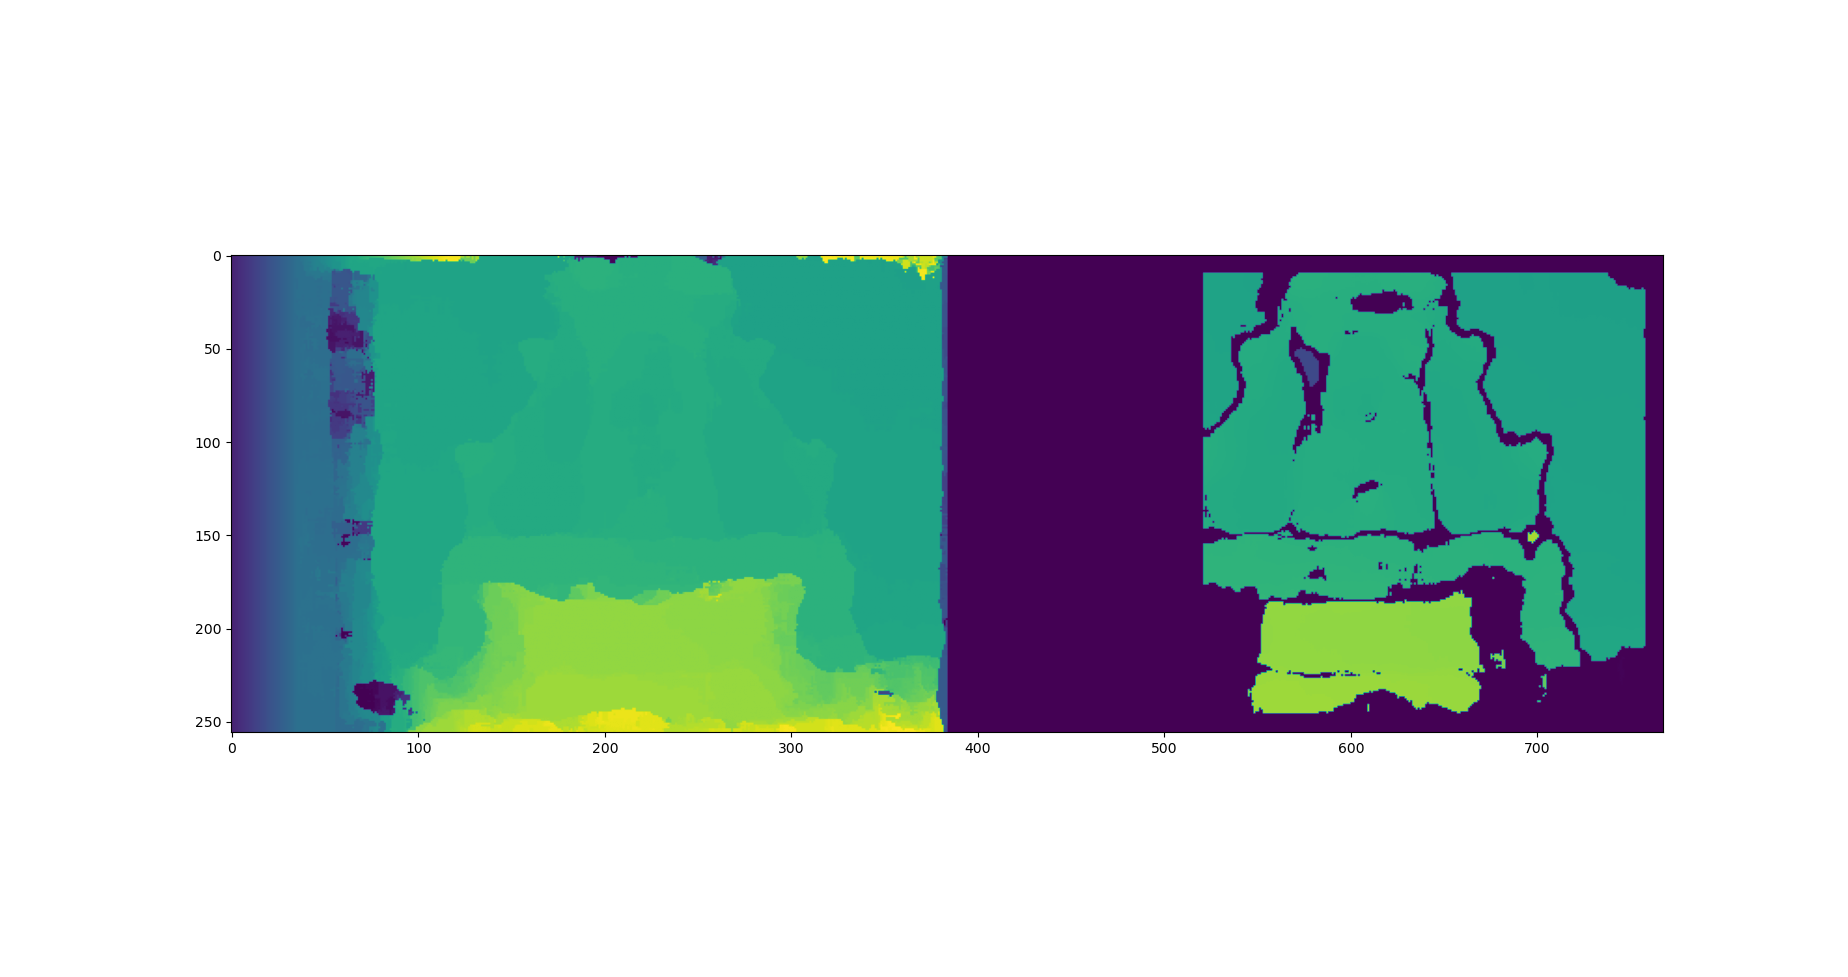
\includegraphics[width=1.0\linewidth]{disparity_comparison.png}
    \caption{Disparity estimates from our implementation (left) and from the off-the-shelf function (right).}
    \label{fig:disparity_comparison}
\end{figure}

A few insights improving the performance of stereo matching are suggested:
\begin{itemize}
    \item Enforce estimated disparity map to be consistent with its neighborhood and change smoothly --- this is because disparity values usually do not change abruptly.
    \item Smooth image pairs before conducting the stereo matching to reduce the impact of image noise.
    \item Conduct SSD calculation over various size of patches and returns the disparity most likely to happen across all block sizes.
\end{itemize}


Also, several conditions favorable to run stereo matching are suggested:
\begin{itemize}
    \item Avoid occulsion in both image pairs.
    \item Rectify image pairs as precise as it could be.
\end{itemize}

I also write code visualizing the estimated disparity maps in 3D coordinates:

\begin{lstlisting}[language=Python, basicstyle=\scriptsize]
# import RGB info pixelwise 
color = (cv2.cvtColor(left_img, cv2.COLOR_BGR2RGB)).astype(np.float64).reshape(-1, 3)

# cast non-positive disparities to nan
disparity[np.where(disparity==-1)] == np.nan
disparity_cv2[np.where(disparity_cv2==-1)] == np.nan

# read baseline and focal length
baseline = np.linalg.norm(t)
f = np.linalg.norm(np.diag(K1)[:-1])

# generate meshgrid in a normalized image coordinate
U, V = np.meshgrid(np.arange(w)-w//2, np.arange(h)-h//2)

fig = plt.figure()

for i, disp in enumerate([disparity, disparity_cv2]):
    # project pointclouds in 3d space upon estimated disparity
    Z = baseline / disp * f
    X = Z / f * U
    Y = -Z / f * V
    
    # create position and corresponding color for projected 3d points
    xyz = np.stack([X,Y,Z], axis=2)
    xyz = np.reshape(xyz, (-1, 3))

    # draw 3d points with corresponding color
    ax = fig.add_subplot(f'12{i+1}', projection='3d')
    ax.scatter(xyz[:, 2], xyz[:, 0], xyz[:, 1], c=color/255.0, label='Points')
    ax.legend(loc='best')
    ax.view_init(azim=-145, elev=30)
    ax.set_xlim((6, 15))
    ax.set_ylim((-5, 5))
    ax.set_zlim((-4, 4))

plt.show()
\end{lstlisting}

Note that the actual distance of a point in a disparity map from the camera (\texttt{Z}) can be reconstructed when the baseline (distance between a pair of cameras taking images) and the focal length are given, which also yields where the corresponding pixel coordinate is projected onto the 3D plane distant from camera by \texttt{Z}. 

Fig.~\ref{fig:disparity2pcd} compares the reconstructed 3D points from the disparity maps estimated by our implementation and the off-the-shelf function, boht of which we obtain in the previous section. Note that the former is imperior to the latter, with lots of noise and outliers.

\begin{figure}[h]
    \centering
    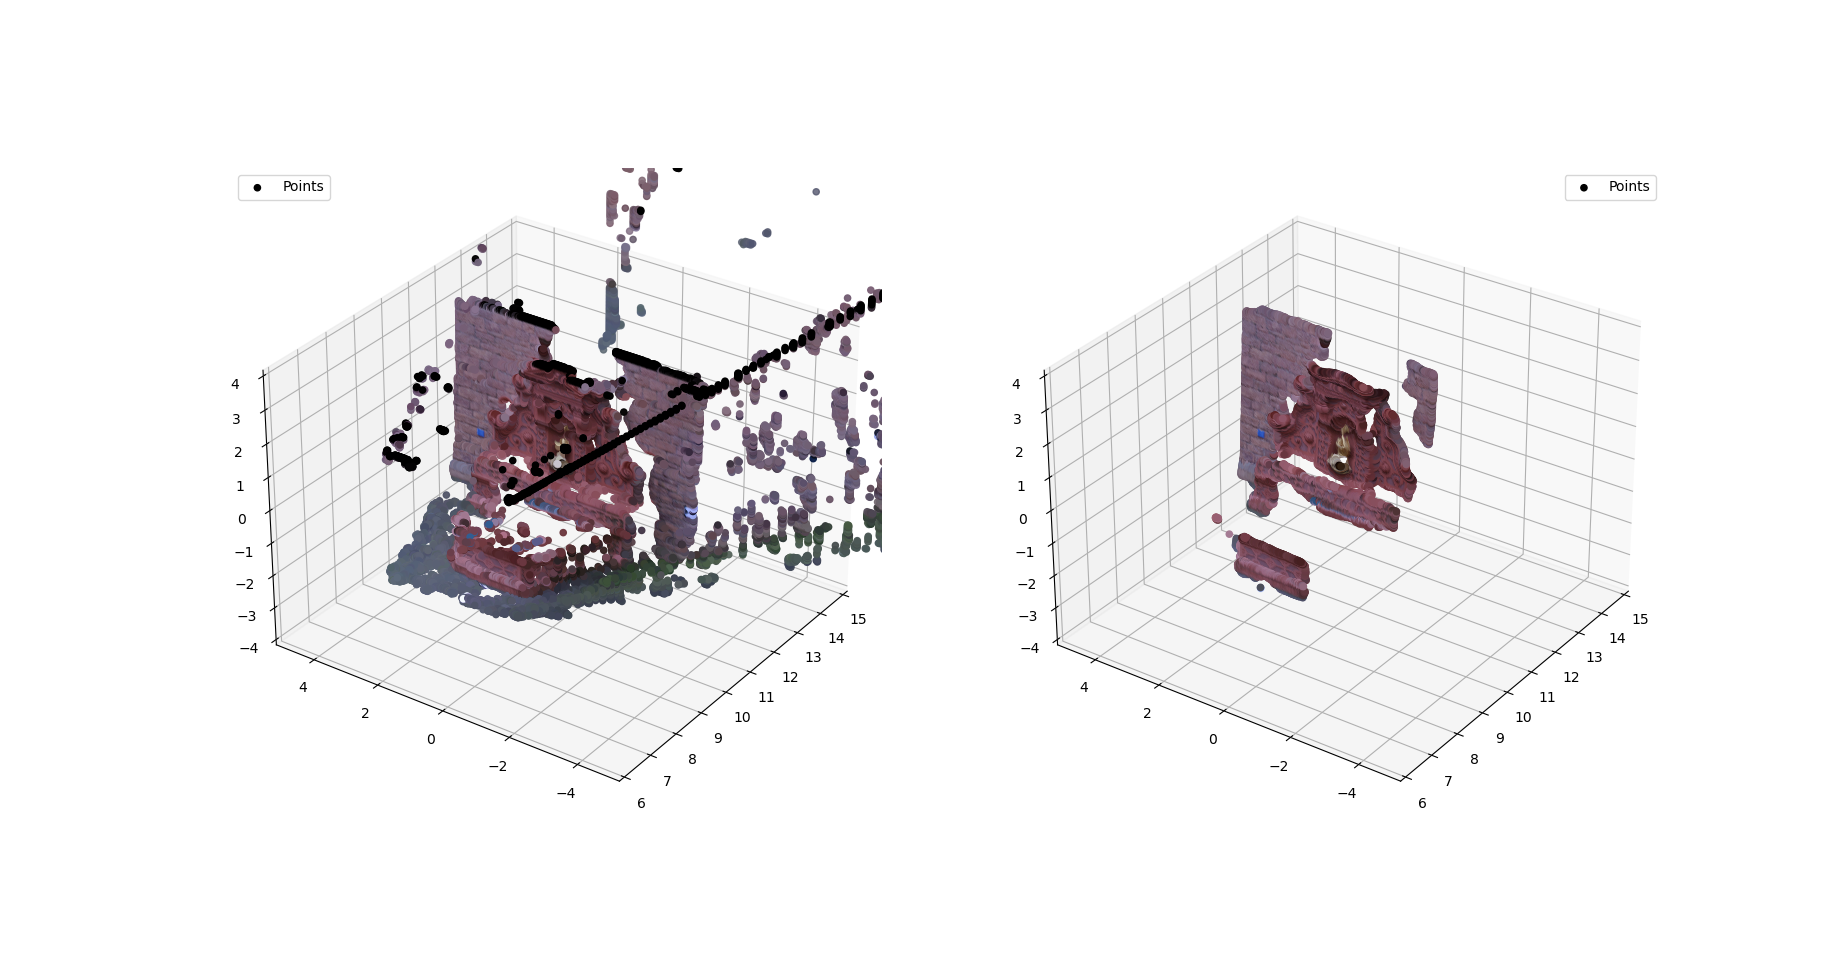
\includegraphics[width=1.0\linewidth]{disparity_to_pointcloud.png}
    \caption{Pointclouds from disparity estimates of our implementation (left) and of the off-the-shelf function (right).}
    \label{fig:disparity2pcd}
\end{figure}

\end{quote}


% \paragraph{Answer:} 
% \begin{quote}
% \end{quote}

% \begin{lstlisting}[language=Python, basicstyle=\scriptsize]
% \end{lstlisting}


% \section*{Bundle Adjustment} 

% \paragraph{Question 6 (Jacobian Calculation) [pt]:}
% # For this question, please use our provided notation, and derive the Jacobian matrix with respect to 3d point $X^i$. We denote the rotation matrix as $R_a$, translation for camera i as $t_a$, intrinsic matrix  as $K_a$ for camera pose a. $x_a^i$ represent the 2d point corresponds to the 3d point $X^i$ in camera pose $a$. In your solution, make sure to give details about how you derive the Jacobian of E with respect to $X_i$.
% \begin{equation*}
%     \begin{split}
%         \underset{X, R, t}{\text{min}} ~E = \underset{i}{\sum} \Vert K_a[R_a | t_a] X^i - x^i_a\Vert
%     \end{split}
% \end{equation*}
% \paragraph{Question 7 (Gaussian Newton Update)~ [pt]:} 
% For this question, please implement your estimated Jacobian for a single 3d point, and implement Gaussian Newton Update step. You are given the initial estimated for 3d point $X^i$, together with ground-truth camera poses $R$, $t$, and camera intrinsics $K$. For simplicity, the bundle adjustment for this problem only optimizes 3d points location $X$. Please report the residual error in your PDF report.

\paragraph{Question 7 (Structure-from-Motion) [bonus 3 pts]:}
We believe you have a thorough understanding of multi-view geometry now. This bonus question will expand the two-view structure-from-motion and stereo estimation problem into multiple views. You have two directions to win the three bonus points: 1) Write your own mini bundle adjustment solver and run it on the fountain dataset. You could leverage Ceres, g2o, GTSAM libraries as your non-linear least square solver, but you need to derive the Jacobian of the energy terms and write your own code to initialize camera poses and 3D points, based on two-view geometry; 2) Collect your own data and utilize Colmap (https://demuc.de/colmap/) to run the full MVS pipeline. This includes correspondences matching, initialization, bundle adjustment, multi-view stereo matching, and depth fusion. Visualize your camera trajectories, sparse point cloud from SFM, and the final dense point cloud from multi-view stereo. Try your best to get the most creative and visually appealing results. We will choose the top solutions in each direction and announce them in the class. 
\end{document}. 

\grid
\grid